%
% grundlagen.tex -- Paper zum Thema Optische Fouriertransformation <opt>
%
% (c) 2023 Marco Niederberger, Yanick Schoch; OST Ostschweizer Fachhochschule
%
% !TEX root = ../../buch.tex
% !TEX encoding = UTF-8
%
\section{Von der Beugung zu Fourier\label{opt:section:grundlagen}}
\rhead{Von der Beugung zu Fourier}

Im folgenden wird der Schritt von der Beugung zur Fouriertransformation vollzogen.
Dazu wird mit der Wellentheorie die Grundlage gelegt für die nachfolgende Herleitung.
Diese gliedert sich anschliessend in drei Abschnitte. 
Zunächst wird das allgemeine Beugungsintegral hergeleitet, das allgemein gültig, aber nicht fundamental lösbar ist.
Anschliessend wird das Integral im Unterkapitel \ref{opt:sec:fresnel} mittels der Fresnel-Approximation für kleine Winkel angenähert.
Eine weitere Vereinfachung wird durch die Linearisierung in $y$ erreicht. 
Diese wird im Unterkapitel \ref{opt:sec:fraunhofer} mit der Fraunhofer-Approximation durchgeführt.

Im Unterkapitel \ref{opt:sec:intensity} wird als letzter Schritt der Zusammenhang zwischen der elektrischen Feldstärke und der Intensität hergestellt.
Denn nur diese kann mit dem Auge oder einem Kamerachip beobachtet werden.

Das Kapitel wird mit einem Rechenbeispiel für die Beugung am Einzelspalt abgeschlossen. 

\subsection{Wellentheorie}
\label{opt:subsection:huygens}
Das Prinzip der optischen Fouriertransformation basiert auf der Beugung von Wellen.
Im folgenden wird die Beugung grob abgehandelt, für eine weitere Behandlung wird auf Kapitel 32 aus dem Physikbuch der HSR \cite{opt:HSR:Physik2} verwiesen.

Qualitativ lässt sich die Beugung mit dem Prinzip von Huygens erklären. 
Abbildung \ref{opt:fig:huygens} zeigt den konzeptionellen Aufbau einer Welle.
Diese lässt sich als Superposition von unendlichen Elementarwellen betrachten.
An jedem Punkt der so entstehenden Wellenfront entsteht eine neue Elementarwelle und daraus wieder eine neue Wellenfront.
Wenn jetzt ein Hindernis die Fortpflanzung der Welle stoppt, bildet sich aus den nicht abgeblockten Elementarwellen eine neue Wellenfront.
Diese ist jetzt jedoch nicht mehr eben, da die generierenden Elementarwellen auf ein endliches Intervall beschränkt sind.

Dieses Phänomen lässt sich beispielsweise auch am Strand beobachten. 
Wenn eine Welle durch eine Öffnung hindurch kommt, breitet sie sich dahinter kreisförmig wieder aus.

\begin{figure}
    \centering
    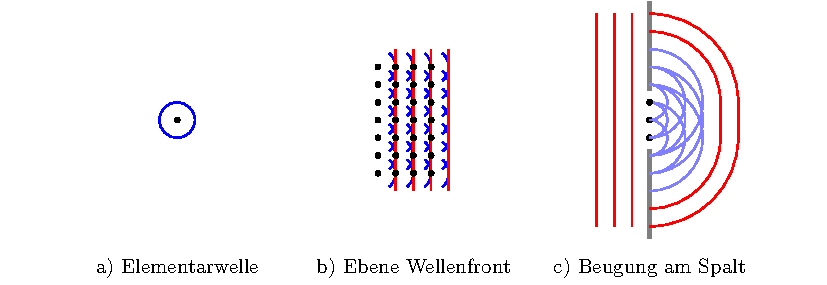
\includegraphics[width=120mm]{papers/opt/images/huygens.pdf}
    \caption{Gemäss dem Prinzip von Huygens kann eine Welle als Summe unendlicher Elementarwellen aufgefasst werden.
    Wenn diese Welle auf ein Hindernis trifft, entsteht dahinter eine neue, gebogene Wellenfront.}
    \label{opt:fig:huygens}
\end{figure}

\subsection{Allgemeines Beugungsintegral}

\begin{figure}
    \centering
    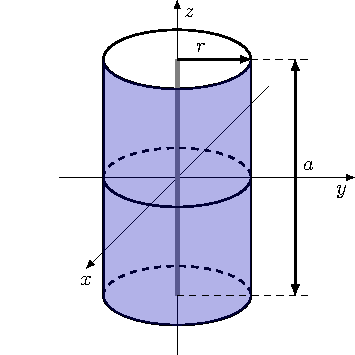
\includegraphics[width=57.34mm]{papers/opt/images/maxwell.pdf}
    \caption{In grau entlang der z-Achse ist die Linienquelle dargestellt, welche vom Zylinder mit dem Radius $r$ und der Länge $a$ umschlossen wird.
    Das elektrische Feld $\vec{E}$ breitet sich immer radial und rechtwinklig zur Lichtquelle aus.}
    \label{opt:fig:maxwell}
\end{figure}

Betrachten wir zuerst, wie in Abbildung~\ref{opt:fig:maxwell} gezeigt, eine unendlich, dünne linienförmige Lichtquelle, welche sich axial in positive und negative z-Richtung unendlich weit erstreckt.
Verallgemeinert kann es sich bei dieser Art von Quelle um eine beliebige elektromagentische Quelle handeln.
Somit kann durch Anwenden der ersten Maxwellschen Gleichung
\begin{equation}
\oint_{S=\partial V} \varepsilon\vec{E} \cdot\, d\vec{S}
=
\int_{V}\rho\, dV
\end{equation}
die elektrische Feldstärke $\vec{E}$ an jedem beliebigen Punkt in Abhängigkeit des radialen Abstandes $r$ berechnet werden.
Dabei ist $\varepsilon$ die dielektrische Feldkonstante, $\rho$ die Ladungsdichte und $V$ das Volumen über dessen Oberfläche $S$ integriert werden muss.
Angewendet auf die gegebene Geometrie des Zylindermantels lässt sich diese Gleichung mittels $\vec{dS} = r d\varphi dl \cdot \hat{r}$ und $\vec{E} = E \cdot \hat{r}$ als
\begin{align}
\int_{0}^{a}\int_{0}^{2\pi} \varepsilon E\cdot \hat{r} \cdot \hat{r} \cdot r\, d\varphi dl
&=
Q
\\
\int_{0}^{a}\int_{0}^{2\pi} \varepsilon E\cdot 1 \cdot r\, d\varphi dl
&=
Q
\\
2\pi ra\varepsilon E
&=
Q
\end{align}
schreiben.
Die durch die Deckflächen entstehenden Randeffekte des elektrischen Feldes können aufgrund der infiniten Länge $a$ des Zylinders vernachlässigt werden.
Wobei es bereits langen würde, wenn $r \ll a$ ist.
Des Weiteren beschreibt $Q$ die durch den Zylindermantel eingeschlossene Ladung.
Zu beachten sei zudem, dass die normierten vektoriellen Grössen $\hat{E} = \hat{r}$ und $\hat{S} = \hat{r}$ parallel verlaufen und sich ihr Skalarprodukt dementsprechend zu 1 vereinfacht.
In anderen Worten, das elektrische Feld $E$ durchtritt die Mantelfläche des Zylinders immer im rechten Winkel.
Nach der elektrischen Feldstärke umgeformt lautet die Gleichung
\begin{equation}
E(r)
=
\frac{Q}{2\pi\varepsilon a} \cdot \frac{1}{r}
=
\theta \cdot \frac{1}{r}
,
\label{opt:equation:E}
\end{equation}
wobei der konstante Anteil als $\theta$ zusammengefasst wurde.

\begin{figure}
    \centering
    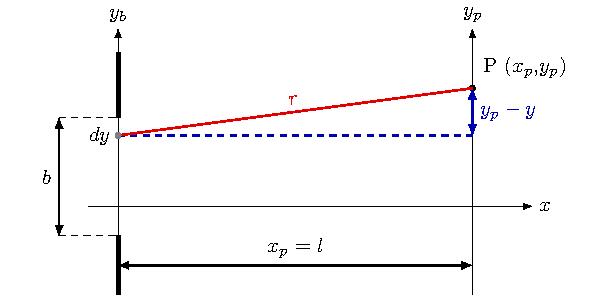
\includegraphics[width=100mm]{papers/opt/images/derivation.pdf}
    \caption{Beugung am Spalt: Die ebene Welle kommt von links her an den Spalt. 
    Von allen $dy$ geht eine Elementarwelle gemäss Kapitel \ref{opt:subsection:huygens} aus, welche sich am Auswertepunkt $P$ aufsummiert.}
    \label{opt:fig:geometricalShape}
\end{figure}

Angenommen eine planare elektromagentische Welle, siehe Abbildung~\ref{opt:fig:geometricalShape}, treffe nun auf eine Blende mit einer unendlich langen und $b$ breiten Öffnung.
Ganz allgemein lässt sich jede Welle als
\begin{equation}
\zeta(x, t)
=
\zeta_0 \cdot e^{j(\omega t - \vec{k}\cdot\vec{x})}
\label{opt:equation:wave}
\end{equation}
ausdrücken.
Wie in Kapitel \ref{opt:subsection:huygens} gezeigt, wird diese Welle an der Blende gebogen.
In Abhängigkeit von der Öffnungsbreite $b$ breitet sich die Welle anschliessend annähernd kreisförmig als neue Wellenfront weiter aus.
Dieses Verhalten der kreisförmigen Ausbreitung kann mittels der zuvor betrachteten Linienquellen modelliert werden.
Infinit viele dieser Linienquellen seien nun nebeneinander entlang der Öffnungsbreite $b$ angereiht.
Die Auswirkung dieser Quellen kann nun an jedem beliebigen Punkt hinter der Blende durch Superposition der einzelnen Quelleneinflüsse berechnet werden.

Ein Schirm werde nun im Abstand $l$ hinter der Blende angebracht, an welchem die elektrische Feldstärke auf verschiedenen Höhen $y_p$ gemessen werden soll.
Aus der geometrischen Anordnung in Abbildung \ref{opt:fig:geometricalShape} geht hervor, dass
\begin{equation}
r
=
\sqrt{l^2 + (y_p-y)^2}
=
l \sqrt{1 + \frac{(y_p-y)^2}{l^2}}
\label{opt:equation:distance_r}
\end{equation}
beträgt. All diese kleinen Einflüsse $dE$ der Linienquellen mit Breite $dy$ superponieren sich, wie bereits erwähnt, zur gesamten elektrischen Feldstärke am Auswertungspunkt.
Ein solcher Einfluss lässt sich nun mittels der Gleichungen~\ref{opt:equation:E} und \ref{opt:equation:wave} als
\begin{equation}
dE
=
E(r) \cdot \zeta(r, t) \cdot dy
=
\frac{\theta}{r} \cdot \zeta_0 \cdot e^{j(\omega t - \vec{k}\cdot\vec{r})} \cdot dy
\end{equation}
beschreiben.
Werden die Einflüsse der Linienquellen über den Spalt integriert, ergibt sich
\begin{equation}
E(y_p, t)
=
\int_{y_b}^{y_b+b}\frac{\theta\zeta_0}{r} \cdot e^{j(\omega t - \vec{k}\cdot\vec{r})} \,dy
=
\theta\zeta_0 \cdot \int_{y_b}^{y_b+b}\frac{e^{j(\omega t - \vec{k}\cdot\vec{r})}}{r} \,dy
.
\end{equation}

Soll nun aber anstelle eines einzelnen Spalts mehrere davon in beliebigen Abständen zueinander betrachtet werden, kann dieses Integral mit Hilfe der Blendenfunktion
\begin{equation}
f(y)
\in
[0, 1]
\end{equation}
dargestellt werden.
Zu beachten ist, dass $f(y)$ nicht nur die Werte 0 und 1, sondern auch jegliche Werte dazwischen annehmen kann.
Dies würde einer teilweise transparenten Blende entsprechen.
Somit folgt als allgemeinste Form
\begin{align}
E(y_p, t)
=
\theta\zeta_0 \cdot \int_{-\infty}^{\infty}f(y)\cdot\frac{e^{j(\omega t - \vec{k}\cdot\vec{r})}}{r} \,dy
.
\label{opt:equation:integral_general}
\end{align}
Dieses Integral ist für jeden Auswertungspunkt allgemein gültig.
Wie sich aber zeigen wird, ist dieses Integral, genauer gesagt $r$ aus Gleichung~\ref{opt:equation:distance_r}, nicht fundamental genug, um es analytisch lösen zu können.
Die folgenden Approximationen von $r$ sollen dabei diese Hürde umgehen.

\subsection{Fresnel-Approximation}
\label{opt:sec:fresnel}
In einer ersten Vereinfachung wird das allgemeine Beugungsintegral aus \ref{opt:equation:integral_general} für kleine Winkel approximiert.
Für weitere Schritte soll die Bedingung
\begin{equation}
y, y_p
\ll
l
\label{opt:equation:condition_fresnel}
\end{equation}
gelten.
Durch Anwenden der Binominalexpansion
\begin{equation}
(1 + \varepsilon)^n
\approx
1 + n\varepsilon
,
\end{equation}
unter der Voraussetzung, dass $\varepsilon \ll 1$ gilt, ist es möglich den Wurzelausdruck aus Gleichung~\ref{opt:equation:distance_r} noch weiter zu vereinfachen.
Mit Hilfe der Vorbedingungen aus Gleichung~\ref{opt:equation:condition_fresnel} ist
\begin{equation}
(y_p-y)^2
\ll
l^2
\end{equation}
gegeben.
Somit kann die Bedingung für
\begin{equation}
\varepsilon
=
\frac{(y_p-y)^2}{l^2}
\ll
1
\label{opt:equation:condition_epsilon}
\end{equation}
eingehalten werden.
Gleichung~\ref{opt:equation:distance_r} vereinfacht sich demnach näherungsweise zu
\begin{equation}
r
=
l \sqrt{1 + \frac{(y_p-y)^2}{l^2}}
\approx
l \left(1 - \frac{(y_p-y)^2}{2l^2}\right)
=
l - \frac{(y_p-y)^2}{2l}
.
\label{opt:equation:distance_r_fresnel}
\end{equation}
Durch Ausklammern von Konstanten und Einsetzen der Gleichung~\ref{opt:equation:distance_r_fresnel} vereinfacht sich das Integral aus Gleichung~\ref{opt:equation:integral_general} weiter zu
\begin{align}
E(y_p, t)
&=
\theta\zeta_0 \cdot e^{j\omega t} \cdot \int_{-\infty}^{\infty}f(y)\cdot\frac{e^{-j\vec{k}\cdot\vec{r}}}{r} \,dy
\\
&=
\theta\zeta_0 \cdot e^{j\omega t} \cdot \int_{-\infty}^{\infty}f(y)\cdot\frac{e^{-jkr \cdot 1}}{r} \,dy
\\
&=
\theta\zeta_0 \cdot e^{j\omega t} \cdot \int_{-\infty}^{\infty}f(y)\cdot\frac{e^{-jkl} \cdot e^{jk\frac{(y_p-y)^2}{2l}}}{l - \frac{(y_p-y)^2}{2l}} \,dy
\\
&=
\theta\zeta_0 \cdot e^{j\omega t} \cdot e^{-jkl} \cdot \int_{-\infty}^{\infty}f(y)\cdot\frac{e^{jk\frac{(y_p-y)^2}{2l}}}{l - \frac{(y_p-y)^2}{2l}} \,dy
.
\end{align}
Wiederum konnte das Skalarprodukt der normierten Grössen $\hat{k}$ und $\hat{r}$ aufgrund Parallelität als 1 gekürzt geschrieben werden.
Des Weiteren kann der Ausdruck $l - \frac{(y_p-y)^2}{2l}$ im Nenner des Integrals als $l$ vereinfacht werden.
Zulässig ist dies nur, weil $(y_p - y)^2 \ll l$ erfüllt ist.
Dasselbe Prinzip darf jedoch nicht auf den Exponenten angewandt werden, da dieser mit dem Faktor der Wellenzahl multipliziert wird und der Term $k \frac{(y_p-y)^2}{2l}$ somit nicht vernachlässigbar klein wird.
Der Zeitpunkt der Auswertung sei nicht von Interesse, da dieser lediglich den Momentanwert der Welle beeinflusst.
Mittels $t = 0$ ergibt sich daraus
\begin{align}
E(y_p, t = 0)
&=
\theta\zeta_0 \cdot e^{j\omega t} \cdot e^{-jkl} \cdot \int_{-\infty}^{\infty}f(y)\cdot\frac{e^{jk\frac{(y_p-y)^2}{2l}}}{l} \,dy
\\
&=
\frac{\theta\zeta_0}{l} \cdot 1 \cdot e^{-jkl} \cdot \int_{-\infty}^{\infty}f(y)\cdot e^{jk\frac{(y_p-y)^2}{2l}} \,dy
\\
&=
\frac{\theta\zeta_0}{l} \cdot e^{-jkl} \cdot \int_{-\infty}^{\infty}f(y)\cdot e^{jk\frac{(y_p^2 - 2y_py + y^2)}{2l}} \,dy
.
\label{opt:equation:integral_fresnel}
\end{align}
Das hiermit erhaltene Integral wird auch als das Fresnel Beugungsintegral bezeichnet und ist in näherer Umgebung um die Blende gültig.

\subsection{Fraunhofer-Approximation}
\label{opt:sec:fraunhofer}
Die Fresnel Approximation aus \ref{opt:equation:integral_fresnel} kann weiter vereinfacht werden.
Dafür wird die Distanz zwischen der Blende und der Auswertungsebene noch weiter erhöht.
Damit wird das möglich, das Integral in Bezug auf die Distanz $y$ zwischen der Quelle und der Auswertungsebene zu linearisieren.
Sei nun
\begin{equation}
y
\ll
y_p
\ll
l
\end{equation}
gegeben, kann der Ausdruck $y_p^2 - 2y_py + y^2$ aus Gleichung~\ref{opt:equation:integral_fresnel} weiter approximiert werden.
Unter Berücksichtigung dieser Bedingung sei $y^2 \ll 2y_py$, wodurch der Term $y^2$ vernachlässigt werden kann.
Daraus folgt
\begin{align}
E(y_p)
&=
\frac{\theta\zeta_0}{l} \cdot e^{-jkl} \cdot \int_{-\infty}^{\infty}f(y)\cdot e^{jk\frac{(y_p^2 - 2y_py)}{2l}} \,dy
\\
&=
\frac{\theta\zeta_0}{l} \cdot e^{-jkl} \cdot e^{jk\frac{y_p^2}{2l}} \cdot \int_{-\infty}^{\infty}f(y)\cdot e^{-jk\frac{y_py}{l}} \,dy
\\
&=
\frac{\theta\zeta_0}{l} \cdot e^{-jk\left(l-\frac{y_p^2}{2l}\right)} \cdot \int_{-\infty}^{\infty}f(y)\cdot e^{-j\frac{ky_p}{l}y} \,dy
.
\label{opt:equation:integral_fraunhofer}
\end{align}
Das somit entstandene Integral entspricht gerade der Fourier-Transformation der Blendenfunktion $f(y)$.

\subsection{Intensität}
\label{opt:sec:intensity}
Die in \ref{opt:equation:integral_fraunhofer} hergeleitete elektrische Feldstärke kann nicht direkt beobachtet werden.
Denn ein Beobachter, sei es das menschliche Auge oder ein Kamera Chip, kann negative und positive Amplituden sowie komplexwertige Grössen nicht unterscheiden.
Gesehen werden kann lediglich die Intensität $I$, welche sich proportional zur elektrischen Feldstärke verhält.
Als Proportionalitätskonstante wird $\kappa$ verwendet.
Woraus sich aus Gleichung~\ref{opt:equation:integral_fraunhofer}
\begin{align}
I(y_p)
&=
\kappa \cdot |E(y_p)|^2
\\
&=
\kappa \cdot \left(\frac{\theta\zeta_0}{l} \cdot 1 \cdot \int_{-\infty}^{\infty}f(y)\cdot e^{-j\frac{ky_p}{l}y} \,dy\right)^2
\\
&=
\kappa \cdot \frac{\theta^2\zeta_0^2}{l^2}\cdot \left(\int_{-\infty}^{\infty}f(y)\cdot e^{-j\frac{ky_p}{l}y} \,dy\right)^2
\label{opt:equation:integral_intensity}
\end{align}
ergibt. Soll nun der exakte Wert von $\kappa$ bestimmt werden, werden weitere Kenntnisse der Elektrotechnik benötigt.
Dieser kann Mittels des Poynting Vectors
\begin{equation}
\vec{S} = \vec{E} \times \vec{H}
\label{opt:equation:poynting}
\end{equation}
hergeleitet werden.
\opttodo{Abbildung von Poynting Vector hinzufügen}
Dabei beschreibt $\vec{E}$ die elektrische und $\vec{H}$ die magnetische Feldstärke.
Angenommen eine elektromagentische Welle breitet sich nun in z-Richtung in einem homogenen Medium aus, was unter anderem bedeutet, dass $\vec{E}$ und $\vec{H}$ immer orthogonal zueinander stehen müssen.
Verläuft nun die elektrische Feldstärke $\vec{E}$ entlang der x-Richtung, muss die magentische Feldstärke $\vec{H}$ entlang der y-Richtung verlaufen.
Diese beiden Quantitäten können wiederum in komplexwertiger Notation, ähnlich zu Gleichung~\ref{opt:equation:wave}, als
\begin{align}
\vec{E}(z,t)
&=
E_0 \cdot e^{j(\omega t-k z)} \cdot \vec{x}
\\
\vec{H}(z,t)
&=
H_0 \cdot e^{j(\omega t-k z)} \cdot \vec{y}
\end{align}
geschrieben werden.
Eingesetzt in Gleichung~\ref{opt:equation:poynting} kann der Ausdruck als
\begin{align}
\vec{S}
&=
\left(E_0 \cdot e^{j(\omega t-k z)} \cdot \vec{x}\right) \times \left(H_0 \cdot e^{j(\omega t-k z)} \cdot \vec{y}\right)
\\
&=
E_0 H_0 \cdot e^{2j(\omega t-k z)} \cdot \vec{z}
\\
&=
E_0 H_0 \cdot \left(\cos{(2(\omega t-kz))}+j\sin{(2(\omega t-kz))}\right) \vec{z}
\end{align}
vereinfacht werden.
Da das zweite Moment des real oder imaginär Teils des Poynting Vectors gerade der gesuchten Intensität $I$ entspricht, kann dieser als 
\begin{align}
I
&=
E(\Re\{S\}^2)
=
E(\Im\{S\}^2)
\\
&=
\frac{1}{t_1- t_0} \int_{t_0}^{t_1} \Re\{S\}^2 \,dt
\\
&=
\frac{1}{t_1 - t_0} \cdot E_0 H_0 \cdot \int_{t_0}^{t_1}\cos\left({2(\omega t-kz)}\right)^2 \,dt
\\
&=
\frac{1}{t_1 - t_0} \cdot E_0 H_0 \cdot \int_{t_0}^{t_1}\frac{\cos(4(\omega t-kz)) + 1}{2} \,dt
\end{align}
geschrieben werden.
Soll nur über die Zeit gemittelt werden, ist die Position $z$ nicht von belangen und kann deshalb auf $z=0$ gesetzt werden.
Beispielsweise kann exakt über eine Periode integriert werden, was in Integrationsgrenzen von $t_0=0$ und
\begin{align}
4\omega t_1
&=
2\pi
\\
t_1
&=
\frac{\pi}{2\omega}
\end{align}
resultiert.
Mit den eingesetzten Grenzen ergibt sich daraus
\begin{align}
I
&=
\frac{1}{\frac{\pi}{2\omega} - 0} \cdot E_0 H_0 \cdot \int_{0}^{\frac{\pi}{2\omega}}\frac{\cos(4(\omega t-k\cdot0)) + 1}{2} \,dt
\\
&=
\frac{\omega}{\pi} \cdot E_0 H_0 \cdot \int_{0}^{\frac{\pi}{2\omega}}\cos(4\omega t) + 1 \,dt
\\
&=
\frac{\omega}{\pi} \cdot E_0 H_0 \cdot \left[\frac{\sin(4\omega t)}{4\omega} + t \right]_{0}^{\frac{\pi}{2\omega}}
\\
&=
\frac{\omega}{\pi} \cdot E_0 H_0 \cdot \left(\frac{\sin(2\pi)}{8\omega} + \frac{\pi}{2\omega}\right)
\\
&=
\frac{\omega}{\pi} \cdot E_0 H_0 \cdot \frac{\pi}{2\omega}
\\
&=
\frac{1}{2} \cdot E_0 H_0
.
\end{align}
Dieser Ausdruck hängt jedoch noch von der magentischen Feldstärke $H_0$ ab.
Um ihn entsprechend auf Gleichung~\ref{opt:equation:integral_intensity} umformen zu können, müssen ein weiteres Mal die Maxwellschen Gleichungen angewandt werden.
Durch Abbildung \opttodo{Abbildung hinzufügen} ist die Umlaufspannung am Rand der Fläche $A$ gegeben durch
\begin{equation}
\oint_{C=\partial A} \vec{E} \cdot\, d\vec{l}
=
E_y(x+\delta x,t) \cdot a - E_y(x,t) \cdot a
.
\end{equation}
Nur Anteile des elektrischen Feldes in y-Richtung sind in diesem Resultat enthalten, da in den übrigen Richtung das Skalarprodukt $\vec{E} \cdot d\vec{l} = 0$ ergibt, unabhängig von der gewählten Kontur $C = \partial A$.

\opttodo{Weiterschreiben}

\subsection{Beispiel einzelner Spalt}
Als einfachstes Beispiel wird die Beugung an ein einem einzelnen Spalt der Breit $b$ durchexerziert.
In diesem Fall beträgt die Blendenfunktion
\begin{equation}
f(y)
=
\left.
\begin{cases}
1 & \text{für } -\frac{b}{2} \leq x \leq \frac{b}{2} \\
0 & \text{sonst}
\end{cases}
\right\}
.
\end{equation}
Mit Hilfe der Eulerschen Identität des Sinus
\begin{equation}
\sin(x) = \frac{e^{jx} - e^{-jx}}{2j}
\end{equation}
und der Definition der $\sinc$ Funktion
\begin{equation}
\sinc(x) = \frac{\sin(x)}{x}
\end{equation}
vereinfacht sich Gleichung~\ref{opt:equation:integral_intensity} demnach zu
\begin{align}
I(y_p)
&=
\kappa \cdot \frac{\theta^2\zeta_0^2}{l^2}\cdot \left(\int_{-\frac{b}{2}}^{\frac{b}{2}}e^{-j\frac{ky_p}{l}y} \,dy\right)^2
\\
&=
\kappa \cdot \frac{\theta^2\zeta_0^2}{l^2}\cdot \left(-\frac{l}{jky_p} \cdot \left[e^{-j\frac{ky_p}{l}y} \right]_{-\frac{b}{2}}^{\frac{b}{2}}\right)^2
\\
&=
\kappa \cdot \frac{\theta^2\zeta_0^2}{l^2}\cdot \left(-\frac{l}{jky_p} \cdot \left[e^{-j\frac{bky_p}{2l}} - e^{-j\frac{bky_p}{2l}}\right]\right)^2
\\
&=
\kappa \cdot \frac{\theta^2\zeta_0^2}{l^2}\cdot \left(-\frac{l}{jky_p} \cdot \left[e^{-j\frac{bky_p}{2l}} - e^{j\frac{bky_p}{2l}}\right]\right)^2
\\
&=
\kappa \cdot \frac{\theta^2\zeta_0^2}{l^2}\cdot \left(\frac{2bl}{bky_p} \cdot \frac{1}{2j} \cdot \left[e^{j\frac{bky_p}{2l}} - e^{-j\frac{bky_p}{2l}}\right]\right)^2
\\
&=
\kappa \cdot \frac{\theta^2\zeta_0^2}{l^2}\cdot \left(\frac{2bl}{bky_p} \cdot \sin\left(\frac{bky_p}{2l}\right)\right)^2
\\
&=
\kappa \cdot \frac{\theta^2\zeta_0^2}{l^2}\cdot b^2 \cdot \sinc^2\left(\frac{bky_p}{2l}\right)
.
\end{align}
